\documentclass{article}
\usepackage{graphicx}
\usepackage{amsmath,amsthm,amssymb}
\usepackage{mdframed}
\usepackage{tikz}
\usepackage{siunitx}
\usepackage{float}
\usepackage{enumitem}
\usepackage{multicol}
\usepackage{esint}
\usepackage{adjustbox}
\usepackage{xcolor}
\usepackage{tcolorbox}
\usepackage[margin=1in]{geometry}
\usepackage[backend=biber, style=numeric]{biblatex}

\definecolor{lightblue}{rgb}{0.89, 0.94, 0.97}
\definecolor{darkblue}{rgb}{0.1, 0.2, 0.6}

\newtcolorbox{graybox}{colframe=black, colback=lightgray, sharp corners, boxrule=0.3mm}

\newtcolorbox{bluebox}{colframe=darkblue, colback=lightblue, sharp corners, boxrule=0.3mm}

\defbibheading{bibliography}{%
  \begin{center}%
    \textsc{\uppercase{\scalebox{1.4}{R}eferences}}%
  \end{center}%
}

\addbibresource{references.bib}

\begin{document}

\begin{titlepage}
   \begin{center}
       \vspace*{1cm}

       \textbf{MATH*4310 Final Project}\\
       The Topology of Planar Graphs

       \vspace{0.5cm}
       
            
       \vspace{0.8cm}

       \text{Finn Steinke}

       \vfill
            
       
            
       \vspace{0.8cm}
            
       Department of Mathematics and Statistics\\
       University of Guelph\\
       Canada\\
       April 17, 2025
            
   \end{center}
\end{titlepage}

\noindent\underline{\textbf{Recall:}} A graph $G = (V,E)$ is said to be \textbf{planar} if there exists a way to embed $G$ in $\mathbb{R}^{2}$, such that no edge, $\{v_{i},v_{j}\} \in E$, intersects with any other edge in $E$, for all $i\neq j$, where $v_{i}, v_{j}\in V$\cite{Fary1948}.\\

\noindent\underline{\textbf{Examples:}}
\begin{multicols}{2}
    \begin{enumerate}[label=(\roman*)]
        \item $Q_{3}$\\\\
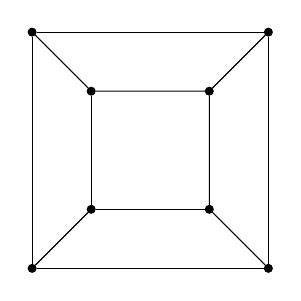
\begin{tikzpicture}[scale=1.5]
\node (v000) at (0,0) [circle, draw, fill=black, inner sep=1pt] {};
\node (v001) at (2,0) [circle, draw, fill=black, inner sep=1pt] {};
\node (v010) at (0,2) [circle, draw, fill=black, inner sep=1pt] {};
\node (v011) at (2,2) [circle, draw, fill=black, inner sep=1pt] {};

% Define the inner square vertices
\node (v100) at (0.5,0.5) [circle, draw, fill=black, inner sep=1pt] {};
\node (v101) at (1.5,0.5) [circle, draw, fill=black, inner sep=1pt] {};
\node (v110) at (0.5,1.5) [circle, draw, fill=black, inner sep=1pt] {};
\node (v111) at (1.5,1.5) [circle, draw, fill=black, inner sep=1pt] {};

% Connect the outer square vertices
\draw (v000) -- (v001);
\draw (v001) -- (v011);
\draw (v011) -- (v010);
\draw (v010) -- (v000);

% Connect the inner square vertices
\draw (v100) -- (v101);
\draw (v101) -- (v111);
\draw (v111) -- (v110);
\draw (v110) -- (v100);

% Connect the inner and outer vertices
\draw (v000) -- (v100);
\draw (v001) -- (v101);
\draw (v010) -- (v110);
\draw (v011) -- (v111);
\end{tikzpicture}\\
        \item $C_{10}$\\\\
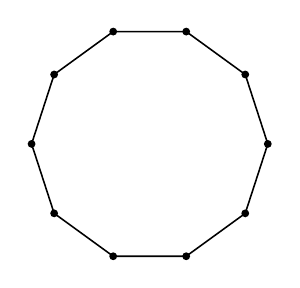
\begin{tikzpicture}

% Draw a decagon with very thin lines and a smaller size
\draw[thick, line width=0.2mm] (0:1.5) -- (36:1.5) -- (72:1.5) -- (108:1.5) -- (144:1.5) -- (180:1.5) -- (216:1.5) -- (252:1.5) -- (288:1.5) -- (324:1.5) -- cycle;

% Add vertices at each corner with smaller size
\foreach \i in {0, 36, 72, 108, 144, 180, 216, 252, 288, 324} {
    \node[fill=black, circle, inner sep=1pt] at (\i:1.5) {};
}

\end{tikzpicture}
    \end{enumerate}
\end{multicols}

\noindent Planar graphs form distinct objects known as \textbf{faces}, of which we can recall a naïve definition from lecture. However, to make the idea of a face more rigorous, we can use certain ideas from topology\cite{Alexander1934}, a pattern that will continue throughout our discussion of planarity. We begin, fittingly, with the definition of a metric space.\\

\begin{graybox}
\noindent\underline{\textbf{Definition:}} Let $x,y,z\in X$, where $X$ is a set. A \textbf{metric space} $(X,d)$ is an ordered pair consisting of $X$ and a function $d:X\times X\to \mathbb{R}$, satisfying the following axioms:
\begin{enumerate}[label=(\roman*)]
  \item $d(x,x) = 0$,
  \item If $x\neq y$, then $d(x,y)>0$,
  \item $d(x,y) = d(y,x)$,
  \item $d(x,z) \leq d(x,y) + d(y,z)$.
\end{enumerate}
The function $d$ is often called the \textbf{metric} or \textbf{distance function}.
\end{graybox}

\noindent Some examples of metric spaces are given below, where we will place a particular emphasis on the third example for our purposes:\\

\noindent\underline{\textbf{Examples:}}
\begin{enumerate}[label=(\roman*)]
    \item
        $\bigl(\mathbb{R}^{n}, ||\cdot||_{\infty}\bigr)$,\\
        
        representing the \textbf{$\ell^{\infty}$-normed space} over $\mathbb{R}^{n}$, where $||\cdot||_{\infty} = \max\limits_{1\leq i\leq n}|x_{i}|$,
    \item
        $\bigl(\mathbb{R}^{n}, ||\cdot||\bigr)$,\\
        representing the \textbf{Euclidean space} $\mathbb{R}^{n}$, where $||\cdot|| =\left( \displaystyle\sum_{i=1}^n |x_i|^2 \right)^{1/2}$,
    \item
        $(V, d_{G})$,\\

        representing the \textbf{graph metric space}, where, if given two vertices $u,v\in V$ connected by a path, then\\ $d_{G}(u,v) = \min\:\{k\in\mathbb{N}\:|\:u=v_{0}\sim v_{1}\sim\cdots\sim v_{k}=v\}$.
\end{enumerate}
Given a planar graph $G = (V,E)$, we can now define $(V, d_{G})$ as our associated metric space, giving us a topological foundation for our graphs. We move directly to the next definition.\\

\begin{graybox}
\noindent\underline{\textbf{Definition:}} A subset $U$ of a metric space $(X, d)$ is called \textbf{open}, if for any point $x\in U$, there exists $\epsilon\in \mathbb{R}$ such that any point $y\in X$ which satisfies $d(x,y)<\epsilon$ belongs to $U$.
\end{graybox}

\noindent To unpack this definition, we commonly use an example in $\mathbb{R}^{2}$, one which is particularly helpful in the context of planar graphs. Let us consider the following example.\\

\noindent\underline{\textbf{Example:}} Consider the metric space $\bigl(\mathbb{R}^{2}, ||\cdot||\bigr)$. Let $U\subseteq \mathbb{R}^{2}$, where $x\in U$. If we can select any $y_{i}\in X$ such that $d(x,y)<\epsilon$, and if we know that the selected $y_{i}\in U$, then we can conclude $U$ is open. This is visually represented by our open circle in $\mathbb{R}^{2}$ shown below:
\begin{figure}[H]
    \centering
    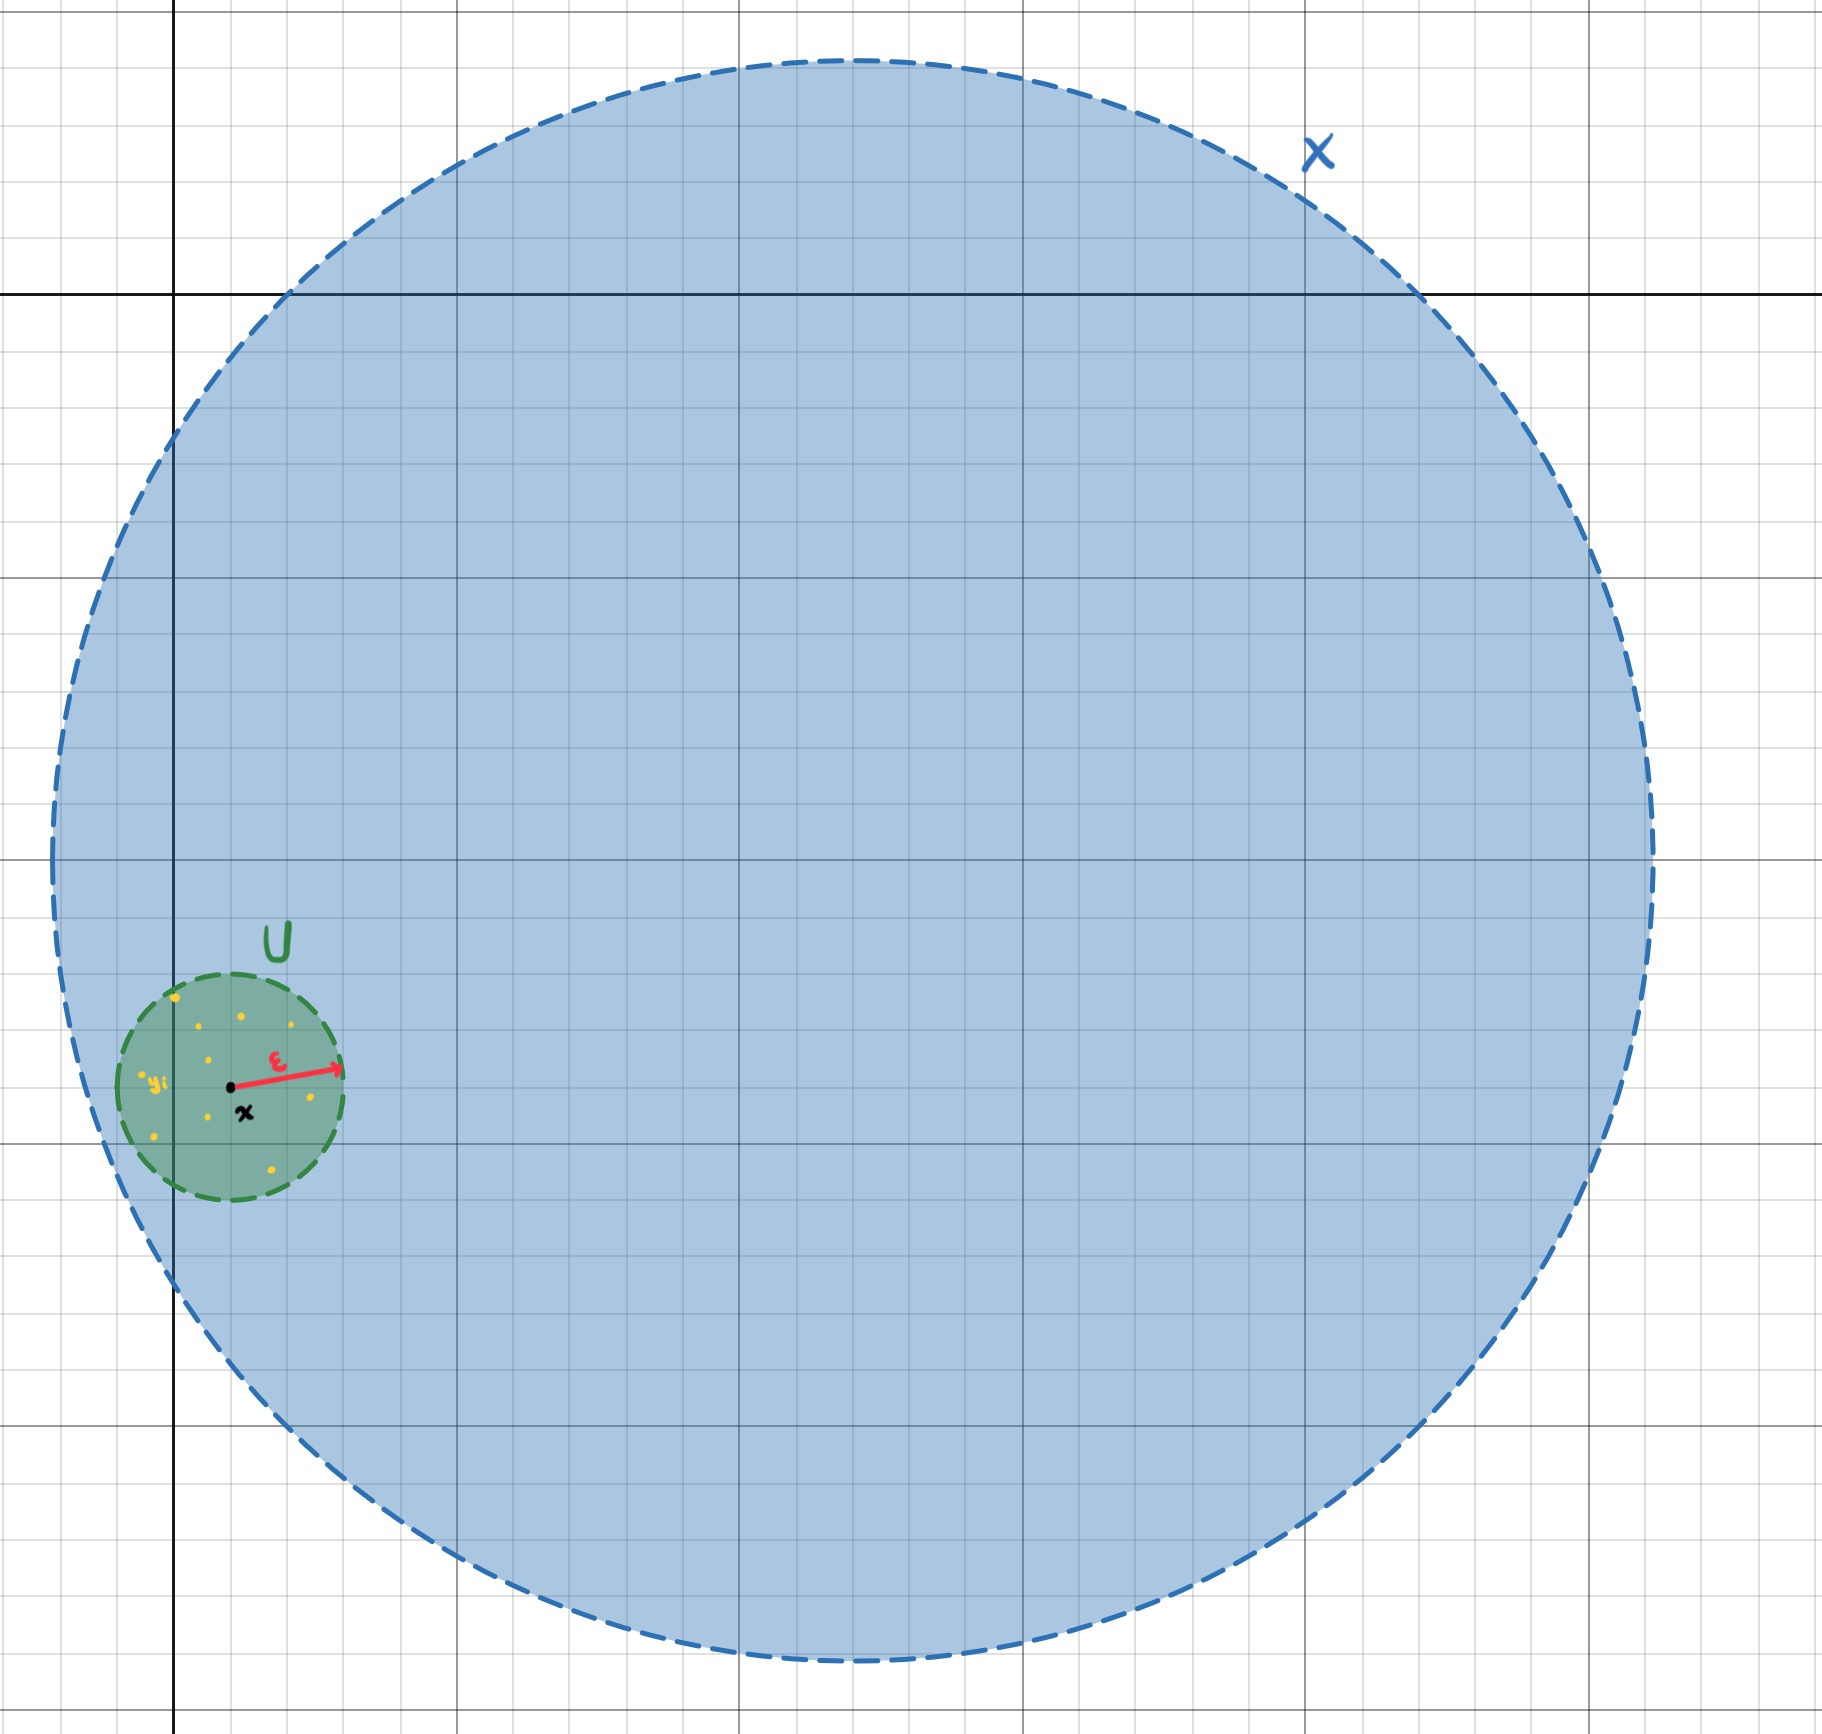
\includegraphics[width=0.8\linewidth]{IMG_0549.jpeg}
\end{figure}
\noindent We see every yellow point $y_{i}$ lies within the boundary of $U$, a circle of radius $\epsilon$, and hence $U$ is open.\\

\noindent Open sets are not limited to subsets of $\mathbb{R}^{n}$, but the particular definition above is useful when touching on the idea of a face in a planar graph, as we will soon see.\\

\noindent We can directly relate our graph metric space and the Euclidean $\mathbb{R}^{2}$ plane through a \textbf{graph embedding}. This process is reliant on a few other topological concepts, and thus we move to understand another definition.

\pagebreak

\begin{graybox}
\noindent\underline{\textbf{Definition:}} Let $X$ be a set, and let $I$ be an arbitrary index set. Then, a \textbf{topological space} is an ordered pair $(X, \mathcal{T})$ consisting of $X$ and a collection of subsets of $X$, $\mathcal{T}$, satisfying the following axioms:
\begin{enumerate}[label=(\roman*)]
  \item $X\in\mathcal{T}$ and $\emptyset\in\mathcal{T}$,
  \item If $\{U_{i}\}_{i\in I} \subseteq\mathcal{T}$, then $\displaystyle\bigcup_{i\in I}U_{i}\in\mathcal{T}$,
  \item If $\{U_{i}\}_{i=1}^{n} \subseteq\mathcal{T}$, then $\displaystyle\bigcap_{i=1}^{n}U_{i}\in\mathcal{T}$.
\end{enumerate}
$\mathcal{T}$ is commonly known as a \textbf{topology} over $X$.
\end{graybox}

\noindent Using the above definitions, we will prove a particularly useful result in the context of metric spaces.\\

\begin{bluebox}
\noindent\underline{\textbf{Theorem.}} \textit{Every metric space $(X,d)$ is a topological space $(X, \mathcal{T})$.}
\end{bluebox}
\begin{proof}
    We will prove this theorem by construction of a topology over $X$.\\

    \noindent Let $(X,d)$ be a metric space, where $d$ satisfies the corresponding axioms of a metric.\\

    \noindent We will construct the \textbf{metric topology} $\mathcal{T}$ of $X$ by defining a collection of open sets of $X$. Let $x\in X$, $\epsilon\in\mathbb{R}\setminus\{0\}$. Then, we define the open ball centred at $x$ as $B_{\epsilon}(x) = \{y\in X\:|\:d(x,y)<\epsilon\}$, where these open balls generate the open sets that form $\mathcal{T}$.

    \begin{enumerate}[label=(\roman*)]
    \item Since $B_{\epsilon}(x)$ is open for any $x\in X$, we know that $\displaystyle\bigcup_{x\in X}B_{\epsilon}(x) = X$. We also know know that $\Biggl(\displaystyle\bigcup_{x\in X}B_{\epsilon}(x)\Biggr)^{C} = \emptyset$, and hence $\emptyset, X\in\mathcal{T}$.

    \item By construction, any arbitrary member of $\bigl\{B_{\epsilon_{i}}(x_{i})\bigr\}_{i\in I}$ in $\mathcal{T}$ will be open and thus $\displaystyle\bigcup_{i\in I}B_{\epsilon_{i}}(x_{i})$ will be open, and thus $\displaystyle\bigcup_{i\in I}B_{\epsilon_{i}}(x_{i}) \in \mathcal{T}$.

    \item Suppose we have $A = B_{\epsilon_{1}}(x_{1})$ and $B = B_{\epsilon_{2}}(x_{2})$, where $A, B \in \mathcal{T}$. Since $A\cap B$ can be covered by a union of smaller $B_{\epsilon_{i}}(x_{i})$, where $\epsilon_{i}<\epsilon_{1}$ and $\epsilon_{i} < \epsilon_{2}$, and where $x_{i} \in A\cap B$, we know that $A\cap B$ will also be open. Hence, any finite number of intersections, $\displaystyle\bigcap_{i=1}^{n}U_{i}\in\mathcal{T}$.
    \end{enumerate}
    Thus, by the definition of a topological space, we can always construct a topology $\mathcal{T}$ on $X$, and therefore the theorem is proven by construction.
\end{proof}

\noindent We will see how useful this theorem is in the following pages.

\pagebreak

\begin{graybox}
\noindent\underline{\textbf{Definition:}} Let $S = (X, \mathcal{T}_{X})$ and $Q = (Y, \mathcal{T}_{Y})$ be topological spaces. A function (or map) $f:X\to Y$ is known as a \textbf{homeomorphism} if it satisfies the following axioms:
\begin{enumerate}[label=(\roman*)]
    \item $f$ is bijective,
    \item $f$ is continuous,
    \item $f^{-1}$ is continuous.
\end{enumerate}

\noindent It is important to note that in the context of topology, two sets $X$ and $Y$ are said to be \textbf{homeomorphic} if a homeomorphism exists between them. This homeomorphism is also an \textbf{equivalence relation}, and hence $X \sim_{R} Y$, where $R$ is also given the symbol "$\cong$".
\end{graybox}

\noindent\underline{\textbf{Examples:}} Some examples of homeomorphisms are as follows:
\begin{enumerate}[label=(\roman*)]
    \item Given $\bigl((0,1), \mathcal{T}_{\text{sub}}\bigr)$ and $(\mathbb{R}, \mathcal{T}_{\text{std}})$, we define $f:(0,1)\to\mathbb{R}$, where $f(x) = \tan\Bigl(\pi x - \dfrac{\pi}{2}\Bigr)$,
    \item Given $(\text{int}\:D^{2}, \mathcal{T}_{D})$ and $(\mathbb{R}^{2}, \mathcal{T}_{\mathbb{R}^{2}})$, we define $f:\text{int}\:D^{2} \to \mathbb{R}^{2}$, where $f(x,y) = \Bigl(\dfrac{x}{1-r^{2}},\:\dfrac{y}{1-r^{2}}\Bigr)$, such that $r^{2} = x^{2} + y^{2}$.
\end{enumerate}

\noindent To preserve the focus on graph theory, we will omit the details of the specific topologies mentioned above, though they have been proven in other texts to be valid.\\

\noindent The next definition will finally solidify our understanding between our combinatorial knowledge and newfound topology knowledge, leading us to a rigorous definition of a graph face.\\

\begin{graybox}
\noindent\underline{\textbf{Definition:}} Let $S = (X, \mathcal{T}_{X})$ and $Q = (Y, \mathcal{T}_{Y})$ be topological spaces. An injective, continuous function (or map) $f:X\to Y$ is called a \textbf{topological embedding} if $X \cong f(X)$.
\end{graybox}

\noindent Given that $G = (V,E)$, we will begin by defining our metric spaces $(V, d_{G})$ and $\bigl([0,1]^{S}, d\bigr)$. We will assume both metric spaces to be valid for the sake of the following definitions, and thus by our theorem above we know each possesses an induced topology. We therefore define the topological embeddings\\
\[\phi: V \to [0,1]^{S},\]
where $V \cong \phi(V)$. However, since the graph $G$ also consists of edges $E$, we must also define the topological embedding 
\[\widehat\phi:E\to [0,1]^{S},\]
where $E \cong \widehat\phi(E)$.\\

\noindent Our final definition before we revisit planar graphs will be a crucial one, but likely also the most vague definition thus far. \textit{(For the sake of the text, we will not discuss the notion of a \textbf{simplicial complex})}.\\

\begin{graybox}
\noindent\underline{\textbf{Definition:}}  
Let $G = (V, E)$ be a graph. We define a topological space $|G|\subseteq [0,1]^{S}$, called the \textbf{geometric realization} of $G$, where $S = V\cup E$. A mapping for a point, $t : S \to [0,1]$, belongs to $|G|$ if and only if it satisfies the following two axioms:
\begin{enumerate}[label=(\roman*)]
    \item The \textbf{support} of \( t \), defined as \( \{s \in S \mid t(s) > 0\} \), is either a singleton \( \{v\} \) for some \( v \in V \), or a pair \( \{u,v\} \) for some edge \( \{u,v\} \in E \).
    \item \( \displaystyle\sum_{s \in S} t(s) = 1 \).
\end{enumerate}
\end{graybox}

\noindent We can now formally define $\phi$ and $\widehat{\phi}$ and prove that there exist valid point mappings to define a geometric realization $|G|$.\\

\begin{bluebox}
\noindent\underline{\textbf{Theorem.}} \textit{Let $G = (V,E)$ be a graph. Then, $\phi: V \to [0,1]^{S}$ and $\widehat{\phi}:E\to[0,1]^{S}$ describe valid topological maps from $G$ to $|G|$.}
\end{bluebox}
\begin{proof}
    We will prove this theorem by construction.\\

    \noindent Let $G = (V,E)$, and let $S = V \cup E$. We define $\phi: V \to [0,1]^S$ to be the map that sends each vertex $v \in V$ to the function $t_v: S \to [0,1]$ defined by
    \[t_v(s) = 
    \begin{cases}
        1 & \text{if } s = v, \\
        0 & \text{otherwise}.
    \end{cases}\]
    Then the support of $t_v$ is $\{v\}$, which is a singleton in $V \subseteq S$, which satisfies condition (i) of the definition of $|G|$. Moreover,
    \[\sum_{s \in S} t_v(s) = t_v(v) = 1,\]
    satisfying condition (ii). Thus, $\phi(v) \in |G|$ for all $v \in V$, and so $\phi$ is well-defined.\\

    \noindent Now, we define $\widehat{\phi}: E \to [0,1]^S$, sending each edge $e = \{u,v\} \in E$ to the function $t_e: S \to [0,1]$ given by
    $$
    t_e(s) =
    \begin{cases}
        \lambda & \text{if } s = u, \\
        1 - \lambda & \text{if } s = v, \\
        0 & \text{otherwise},
    \end{cases}
    $$
    for some fixed $\lambda \in (0,1)$. Then the support of $t_e$ is $\{u,v\} \in E \subseteq S$, and
    $$
    \sum_{s \in S} t_e(s) = \lambda + (1 - \lambda) = 1,
    $$
    satisfying both conditions of the geometric realization.\\

    \noindent Therefore, both $\phi$ and $\widehat{\phi}$ define valid topological maps into $|G|$.
\end{proof}

\noindent With this theorem proven, we will revisit our definition of a planar graph to incorporate all of these topological concepts.\\

\begin{graybox}
\noindent\underline{\textbf{Definition:}} Let $G = (V,E)$ be a finite, simple graph, with geometric realization $|G|$. Then, $G$ is called \textbf{planar} if there exists a topological embedding
\[\Phi:|G| \hookrightarrow \mathbb{R}^{2}.\]
\end{graybox}

\noindent This is the framework for any planar graph and the notion of "embedding" in graph theory\cite{Diestel2005}. Without too large a digression into the topological details, we require the intermediate realization $|G|$ as a topological space, since $G$ has too \textbf{coarse} a topology to directly map to $\mathbb{R}^{2}$ in any "meaningful" way. Generally, we want to capture a more "smooth" map from $|G|$ to $\mathbb{R}^{2}$ than is possible from $G$ to $\mathbb{R}^{2}$.\\

\noindent We follow this with the formal definition of a face in a planar graph. The general idea of the definition is more important than understanding the topological specifics, as they require knowledge of \textbf{homotopy theory}, a topic far beyond the scope of this text.

\pagebreak

\begin{graybox}
\noindent\underline{\textbf{Definition:}} Let $G = (V,E)$ be a planar graph such that $v\in V$ and $e\in E$, where $|G|$ is the geometric realization of $G$. By the definition of a planar graph, we know that $\Phi(v)\in\mathbb{R}^{2}$ for all $v$, and $\Phi(e) \in C^{0}(\mathbb{R}^{2})$ for all $e$, where $\Phi:|G| \hookrightarrow \mathbb{R}^{2}$. A \textbf{face} of $G$ is a \textbf{path-connected component} of $|G|^{C} \subset \mathbb{R}^{2}$, where the faces $F$ form the set
\[F = \pi_{0}\Bigl(\mathbb{R}^{2}\setminus \Phi\bigl(|G|\bigr)\Bigr),\]
where $\pi_{0}(X)$ describes the \textbf{0th homotopy "group"}\footnotemark{} of a set $X$, or set of path-connected components of $X$, assuming $(X, \mathcal{T})$ is a topological space.
\end{graybox}

\footnotetext{$\pi_0$ is not necessarily a group.}


\noindent This definition is quite atrocious. We can gain more insight here by considering the open sets bounded by $\Phi(e)$, where the idea of path-connectedness is more intuitive: these open subsets of $\mathbb{R}^{2}$, simply put, must be simply connected, with one exception.\\

\noindent\underline{\textbf{Example:}} Consider the planar $C_{4}$ embedding below:\\

\begin{center}
% Square graph (C4)
\begin{adjustbox}{valign=c}
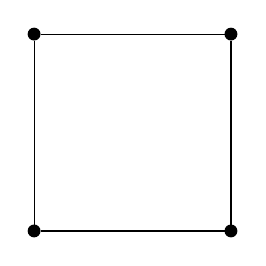
\begin{tikzpicture}
  \foreach \i/\x/\y in {1/0/0, 2/2.5/0, 3/2.5/2.5, 4/0/2.5}
    \node[draw, fill=black, circle, inner sep=1.5pt] (v\i) at (\x,\y) {};

  \draw (v1) -- (v2) -- (v3) -- (v4) -- (v1);
\end{tikzpicture}
\end{adjustbox}
\hspace{1cm}
% Arrow with Phi
\begin{adjustbox}{valign=c}
\(\overset{\Phi}{\longrightarrow}\)
\end{adjustbox}
\hspace{1cm}
% Image
\begin{adjustbox}{valign=c}
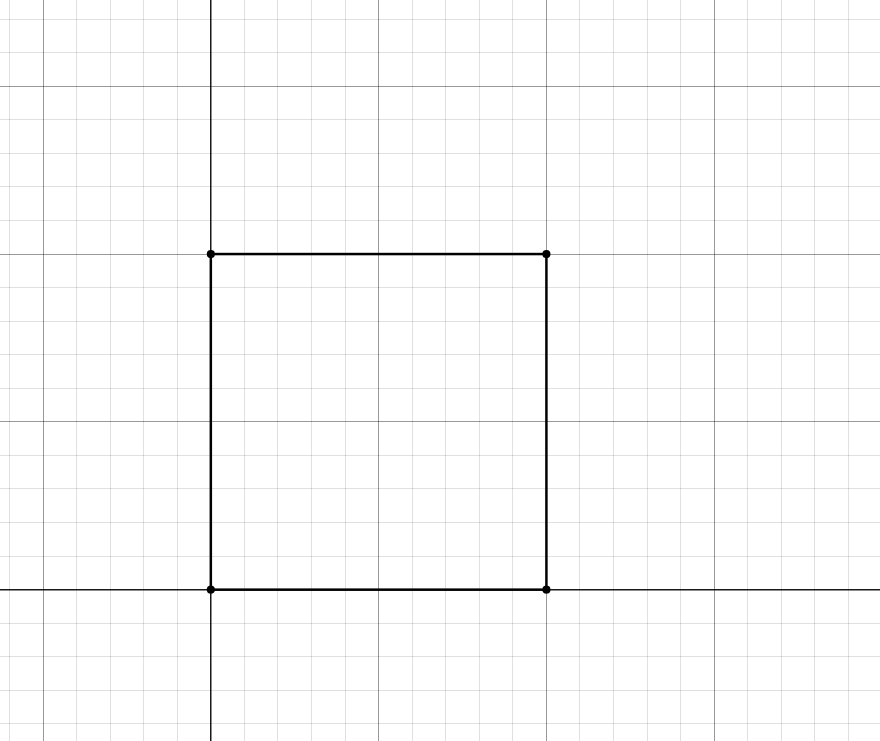
\includegraphics[width=0.42\linewidth]{Screenshot 2025-04-14 200629.png}
\end{adjustbox}
\end{center}

\noindent We find one such simply connected region, \textit{inside} the square region formed by the graph embedding in $\mathbb{R}^{2}$. However, this graph embedding contains \textit{two} faces, not just one. This requires a digression on the aforementioned "one exception".\\

\noindent The formal definition above actually allows for one more face in the planar embedding of any graph, namely the outside, unbounded face. While we consider this a consequence of the topological definition of a face, we can make this inclusion more intuitive.\\

\noindent We consider the topological embedding
\[\Phi':\Phi\bigl(|G|\bigr)\hookrightarrow S^{2},\]
where $S^{2}$ is the $2$-sphere. The reason for this mapping will become clear soon, though it is admittedly not obvious at the moment. To avoid notational clutter, we will also let $\Psi\bigl(|G|\bigr) = \Phi'\circ\Phi\bigl(|G|\bigr)$.\\

\noindent We choose to embed $G$ into $S^{2}$ for a very important reason, which can be explained with a few topological details, beginning with a definition.

\pagebreak

\begin{graybox}
\noindent\underline{\textbf{Definition:}} Let $(X, \mathcal{T})$ be a topological space. Consider the set $X^{*} = X\cup\{\infty\}$, given a topology $\mathcal{C}$, consisting of the open sets of $X$ and, additionally, all subsets $U \subseteq X^{*}$ such that $X^{*}\setminus U$ is \textbf{compact}\footnotemark{} in $X$. Then, $(X^{*}, \mathcal{C})$ is a topological space known as the \textbf{Alexandroff extension}.
\end{graybox}

\footnotetext{Please see any introductory analysis or topology text for the definition of compactness.}

\noindent For the sake of the text, we will assume $\mathcal{C}$ to be a valid topology without providing an explicit proof.\\

\noindent\underline{\textbf{Example:}} Consider the topological space $(\mathbb{R}^{2}, \mathcal{T}_{\mathbb{R}^{2}})$. The Alexandroff extension of this space, $\bigl(\mathbb{R}^{2} \cup \{\infty\}, \mathcal{C}\bigr)$ is visually represented below:

\begin{center}
\begin{adjustbox}{valign=c}
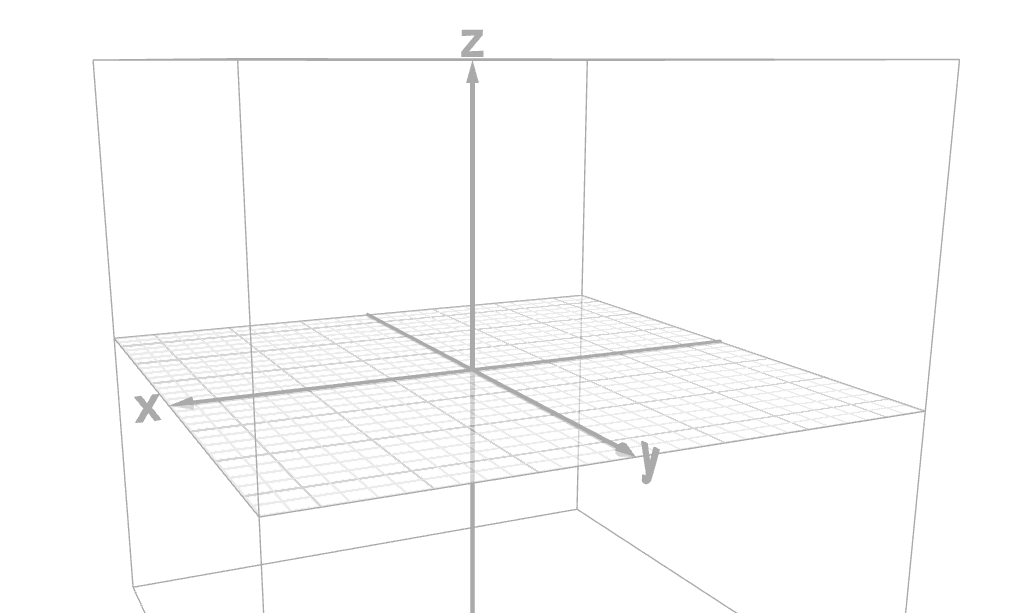
\includegraphics[width=0.45\textwidth]{Screenshot 2025-04-14 211314.png}
\end{adjustbox}
\hspace{0.2cm}
\begin{adjustbox}{valign=c}
\({\longrightarrow}\)
\end{adjustbox}
\hspace{0.2cm}
\begin{adjustbox}{valign=c}
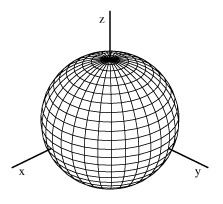
\includegraphics[width=0.45\textwidth]{rcoordsurface-ezgif.com-gif-to-jpg-converter.jpg}
\end{adjustbox}
\end{center}

\noindent This process is also known as the \textbf{one-point compactification} of $\mathbb{R}^{2}$.\\

\noindent The example above is a very important Alexandroff extension for our discussion of the unbounded face in our planar graphs. To show why this is, we begin with a theorem.\\

\footnotetext[3]{Please see any introductory complex analysis text for the definition of a stereographic projection.}

\begin{bluebox}
\noindent\underline{\textbf{Theorem.}} \textit{Let $\bigl(\mathbb{R}^{2} \cup \{\infty\}, \mathcal{C}\bigr)$ be the Alexandroff extension of $(\mathbb{R}^{2}, \mathcal{T}_{\mathbb{R}^{2}})$. Then, $\mathbb{R}^{2} \cup \{\infty\} \cong S^{2}$.}
\end{bluebox}
\begin{proof}
    We will prove this theorem by constructing an explicit homeomorphism from $\mathbb{R}^{2} \cup \{\infty\}$ to $S^{2}$.\\
    
    \noindent Let $S^{2} \subset \mathbb{R}^{3}$ denote the 2-sphere centered at the origin with radius $1$, and let $n = (0,0,1)$ denote the north pole. Define the \textbf{stereographic projection}\footnotemark{} map
    \[\psi : S^{2} \setminus \{n\} \longrightarrow \mathbb{R}^{2}\]
    which is known to be a homeomorphism.\\
    
    \noindent We now define a map
    \[
    \overline{\psi}^{-1} : \mathbb{R}^{2} \cup \{\infty\} \longrightarrow S^{2}
    \]
    given by
    \[\overline{\psi}^{-1}(x,y) = \psi^{-1}(x,y),\]
    for all $(x,y) \in \mathbb{R}^{2}$, and 
    \[\overline{\psi}^{-1}(\infty) = n.\]

    \noindent Since $\psi$ is a homeomorphism, the extension map $\overline{\psi}^{-1}$ is continuous at all points of $\mathbb{R}^{2}$. To check continuity at $\infty$, we note that the neighbourhoods of $\infty$ in the Alexandroff extension are complements of compact sets in $\mathbb{R}^{2}$. The image of these sets under $\overline{\psi}^{-1}$ are open neighbourhoods of $n$ in $S^{2}$, since every neighbourhood of $n$ in $S^{2}$ contains the image of all but a compact subset of $\mathbb{R}^{2}$.\\
    
    \noindent Hence, $\overline{\psi}^{-1}$ is continuous, bijective, and has a continuous inverse. Therefore, it is a homeomorphism.\\
    
    \noindent Therefore, we conclude that
    \[\mathbb{R}^{2} \cup \{\infty\} \cong S^{2}.\]
\end{proof}

\noindent Since we have shown that an Alexandroff extension of $\mathbb{R}^{2}$ will be homeomorphic to $S^{2}$, we reconsider our embedding $\Psi$. As we embed $G$ into $S^{2}$, we find that $\Psi(e) \in C^{0}(S^{2})$ for all $e\in E$. However, as $S^{2}$ is a bounded surface, we also notice that the unbounded face in $\mathbb{R}^{2}$ is now, in fact, bounded in $S^{2}$. Using our previous example of the planar embedding of $C_{4}$, we can visualize this clearly (with a projection):

\begin{center}
% Square graph (C4)
\begin{adjustbox}{valign=c}
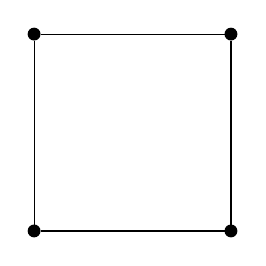
\begin{tikzpicture}
  \foreach \i/\x/\y in {1/0/0, 2/2.5/0, 3/2.5/2.5, 4/0/2.5}
    \node[draw, fill=black, circle, inner sep=1.5pt] (v\i) at (\x,\y) {};

  \draw (v1) -- (v2) -- (v3) -- (v4) -- (v1);
\end{tikzpicture}
\end{adjustbox}
\hspace{1cm}
% Arrow with Phi
\begin{adjustbox}{valign=c}
\(\overset{\Psi}{\longrightarrow}\)
\end{adjustbox}
\hspace{1cm}
% Image
\begin{adjustbox}{valign=c}
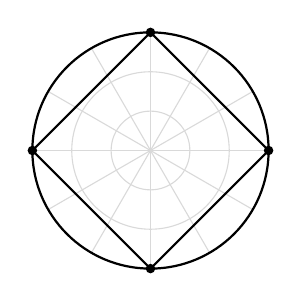
\begin{tikzpicture}

  % Draw faint polar grid
  \foreach \angle in {0,30,...,330} {
    \draw[gray!30, thin] (0,0) -- ({1.5*cos(\angle)}, {1.5*sin(\angle)});
  }
  \foreach \r in {0.5,1.0,1.5} {
    \draw[gray!30, thin] (0,0) circle (\r);
  }

  % Draw outer sphere outline
  \draw[thick] (0,0) circle (1.5cm);

  % Place and draw the vertices and edges of C_4
  \foreach \angle/\name in {0/A, 90/B, 180/C, 270/D} {
    \coordinate (\name) at ({1.5*cos(\angle)}, {1.5*sin(\angle)});
    \filldraw[black] (\name) circle (1.5pt);
  }

  \draw[thick] (A) -- (B) -- (C) -- (D) -- (A);

\end{tikzpicture}
\end{adjustbox}
\end{center}

\noindent Since every $\Phi(e)$ in this embedding borders two faces on the surface $S^{2}$, we finally gain a visual intuition on the previously exceptional case for our planar embedding $\Phi$. All faces are bounded with this embedding, making it a more intuitive embedding to work with. We will also find it is beneficial as we move to understand the next few concepts.\\

\begin{graybox}
\noindent\underline{\textbf{Definition:}} Let $G = (V,E,F)$ be a planar graph with the geometric realization $|G|$, and let\\ $\Psi:|G| \hookrightarrow S^{2}$ be the corresponding embedding. Then, a graph $G^{*} = (V^{*}, E^{*}, F^{*})$ is called the \textbf{dual} of $G$ if it satisfies the following axioms:
\begin{enumerate}[label=(\roman*)]
    \item For all $f \in F$, there exists $v_f^* \in V^*$, placed in the relative interior of $\Psi(f) \subset S^2$,
    \item For all $\{u, v\} \in E$, there exists $e^* \in E^*$, where $e^*$ connects the dual vertices corresponding to the faces adjacent to $\{u, v\}$. The dual edge $e^*$ intersects $\Psi(e)$ exactly once and lies in the interior of $\Psi(e)$,
    \item $|F| = |V^*|$.
\end{enumerate}
\end{graybox}

\pagebreak

\noindent\underline{\textbf{Example:}} Consider the graph below and its dual:

\begin{center}
\begin{adjustbox}{valign=c}
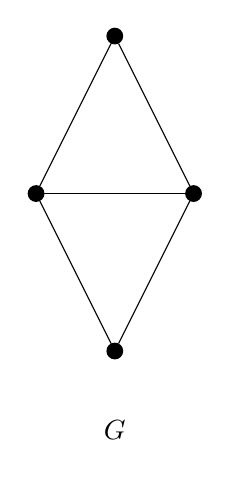
\begin{tikzpicture}
% Vertices
\node[draw, fill=black, circle, inner sep=2pt] (A) at (0,0) {};
\node[draw, fill=black, circle, inner sep=2pt] (B) at (2,0) {};
\node[draw, fill=black, circle, inner sep=2pt] (C) at (1,2) {};
\node[draw, fill=black, circle, inner sep=2pt] (D) at (1,-2) {};

% Edges
\draw (A) -- (B);
\draw (B) -- (C);
\draw (C) -- (A);
\draw (A) -- (D);
\draw (D) -- (B);

% Label for the graph G
\node at (1,-3) {$G$};
\end{tikzpicture}
\end{adjustbox}
\hspace{0.2cm}
\begin{adjustbox}{valign=c}
\({\longrightarrow}\)
\end{adjustbox}
\hspace{0.2cm}
\begin{adjustbox}{valign=c}
\begin{tikzpicture}
% Invisible label at top to force vertical space
\node[text=white] at (1.5, 1.2) {placeholder};

% Dual Vertices
\node[draw, fill=black, circle, inner sep=2pt] (v1) at (0.5, 0.5) {};
\node[draw, fill=black, circle, inner sep=2pt] (v2) at (1.5, 0.5) {};
\node[draw, fill=black, circle, inner sep=2pt] (v3) at (1.5, -2) {};

% Dual Edges
\draw (v1) -- (v2);
\draw (v2) -- (v3);
\draw (v3) -- (v1);

% Label for G^*
\node at (1.5,-3.8) {$G^{*}$};
\end{tikzpicture}
\end{adjustbox}
\end{center}

\noindent While we are familiar with the dual from lecture, we now have the topological understanding of the dual as a construction that depends on the embedding of a graph into a surface. In this sense, graph duality is not purely combinatorial — it is determined by the way the graph sits inside the surface, or in other words, the embedding. Different embeddings can lead to different duals, highlighting the fundamentally topological nature of this construction.\\

\noindent Ultimately, through the discussion of planarity and graph embeddings, we have neglected to mention perhaps the most interesting concept tying the fields of combinatorics and topology together. In order to understand this concept, we must consider the following definition.\\

\begin{graybox}
\noindent\underline{\textbf{Definition:}} Let $G = (V,E,F)$ be a planar graph. Then, the \textbf{Euler characteristic} of $G$ is defined as
\[\chi = |V| - |E| + |F|.\]
\end{graybox}

\noindent This definition leads us to a very important theorem in the context of planar graphs.\\

\begin{bluebox}
\noindent\underline{\textbf{Theorem.}} \textit{Let $G = (V,E,F)$ be a graph. If $G$ is planar, then $\chi = 2$.}
\end{bluebox}
\begin{proof}
    Completed in lecture.
\end{proof}

\noindent While this theorem is a powerful result in combinatorics, it has a much more subtle implication for the topology of our aforementioned graph embeddings. We move to our final definition.\\

\begin{graybox}
\noindent\underline{\textbf{Definition:}} A \textbf{topological invariant} is a property of a topological space that is preserved under homeomorphism.
\end{graybox}

\noindent\underline{\textbf{Example:}} Under any homeomorphisms of our planar graph embeddings, $\chi$ does not change, and hence is a topological invariant.

\pagebreak

\noindent Finally, we arrive at the final theorem of this text\cite{DoCarmo1976}. A rigorous understanding of this theorem is impossible without extensive knowledge of differential topology and geometry, and thus the final section will be brief and less concrete.\\

\begin{bluebox}
\noindent\underline{\textbf{(Gauss-Bonnet) Theorem.}} \textit{Let $M$ be a compact two-dimensional Riemannian manifold with boundary $\partial M$. Let $K$ be the Gaussian curvature of $M$, and let $k_{g}$ be the geodesic curvature of $\partial M$. Then,
\[\int_{M}K\:\mathrm{d}A + \int_{\partial M}k_{g}\:\mathrm{d}s = 2\pi\chi(M),\]
where $\chi(M)$ is the Euler characteristic of $M$.}
\end{bluebox}
\begin{proof}
    Omitted.
\end{proof}

\noindent We will not discuss manifolds, Riemannian geometry, or curvature.\\

\noindent This theorem, however, also uses the Euler characteristic, though not of a graph. This is surprisingly quite a direct connection to graph theory, though will require some reworking of the theorem to adapt its effectiveness in discrete settings.\\

\noindent One common analogous formulation of the Gauss-Bonnet theorem for triangulated surfaces is given below:

\begin{bluebox}
\noindent\underline{\textbf{Theorem.}} \textit{Let $M$ be a finite two-dimensional pseudo-manifold. Let $\chi(v)$ denote the number of triangles containing the vertex $v$. Then,}
\[\sum_{v\in\:\text{int}\:M}\bigl(6-\chi(v)\bigr) + \sum_{v\in\partial M}\bigl(3-\chi(v)\bigr) = 6\chi(M),\]
\textit{where $\chi(M)$ is the Euler characteristic of $M$.}
\end{bluebox}
\begin{proof}
    Omitted.
\end{proof}

\noindent We recall all our previous work towards topological embeddings and specifically $\Psi$, which we used to embed a planar graph $G$ into $S^{2}$. Suppose we have $K_{3}$, and we use the embedding $\Psi(K_{3})$. If we ignore the details required in order to define a proper \textbf{pseudo-manifold}, we will naïvely let $M = S^{2}$. Then, knowing that $\partial M = \emptyset$ (since $S^{2}$ has no boundary), we find that $\chi(v) = 2$ for $\Psi(K_{3})$, and thus
\begin{align*}
    \sum_{v\in\:\text{int}\:S^{2}}(6 - 2) + 0 &= 6\bigl(\chi(S^{2})\bigr)\\
    12 &= 6\bigl(\chi(S^{2})\bigr)\\
    \chi(S^{2}) &= 2,
\end{align*}
where we find the Euler characteristic of $S^{2}$ to be the same as that of a planar graph. This is not an accident and indeed a direct connection between the embedding $\Psi$ and the smooth structure $S^{2}$.\\

\noindent In fact, using the knowledge that for $S^{2}$, $K = \dfrac{1}{r^{2}}$, we can use the general form of Gauss-Bonnet to rearrange for the same result, where
\begin{align*}
    \int_{S^{2}}\frac{1}{r^{2}}\:\mathrm{d}A &= 2\pi\chi(S^{2})\\
    \frac{1}{r^{2}}\int_{S^{2}}\mathrm{d}A &= 2\pi\chi(S^{2})\\
    \frac{1}{r^{2}}(4\pi r^{2}) &= 2\pi\chi(S^{2})\\
    \chi(S^{2}) &= 2.
\end{align*}
This theorem encodes a beautiful connection between planar graph embeddings and the smooth manifold we embedded the graphs on, where $\chi(G) = \chi(S^{2})$, displaying a clear example of a topological invariant. This is a rare case where we can create a direct link between discrete and continuous, and displays a wonderful harmony between combinatorics and topology.

\pagebreak



\printbibliography

\end{document}
